\chapter{Prototype Axion Detectors}

\begin{figure}[htb] 
    \centering
    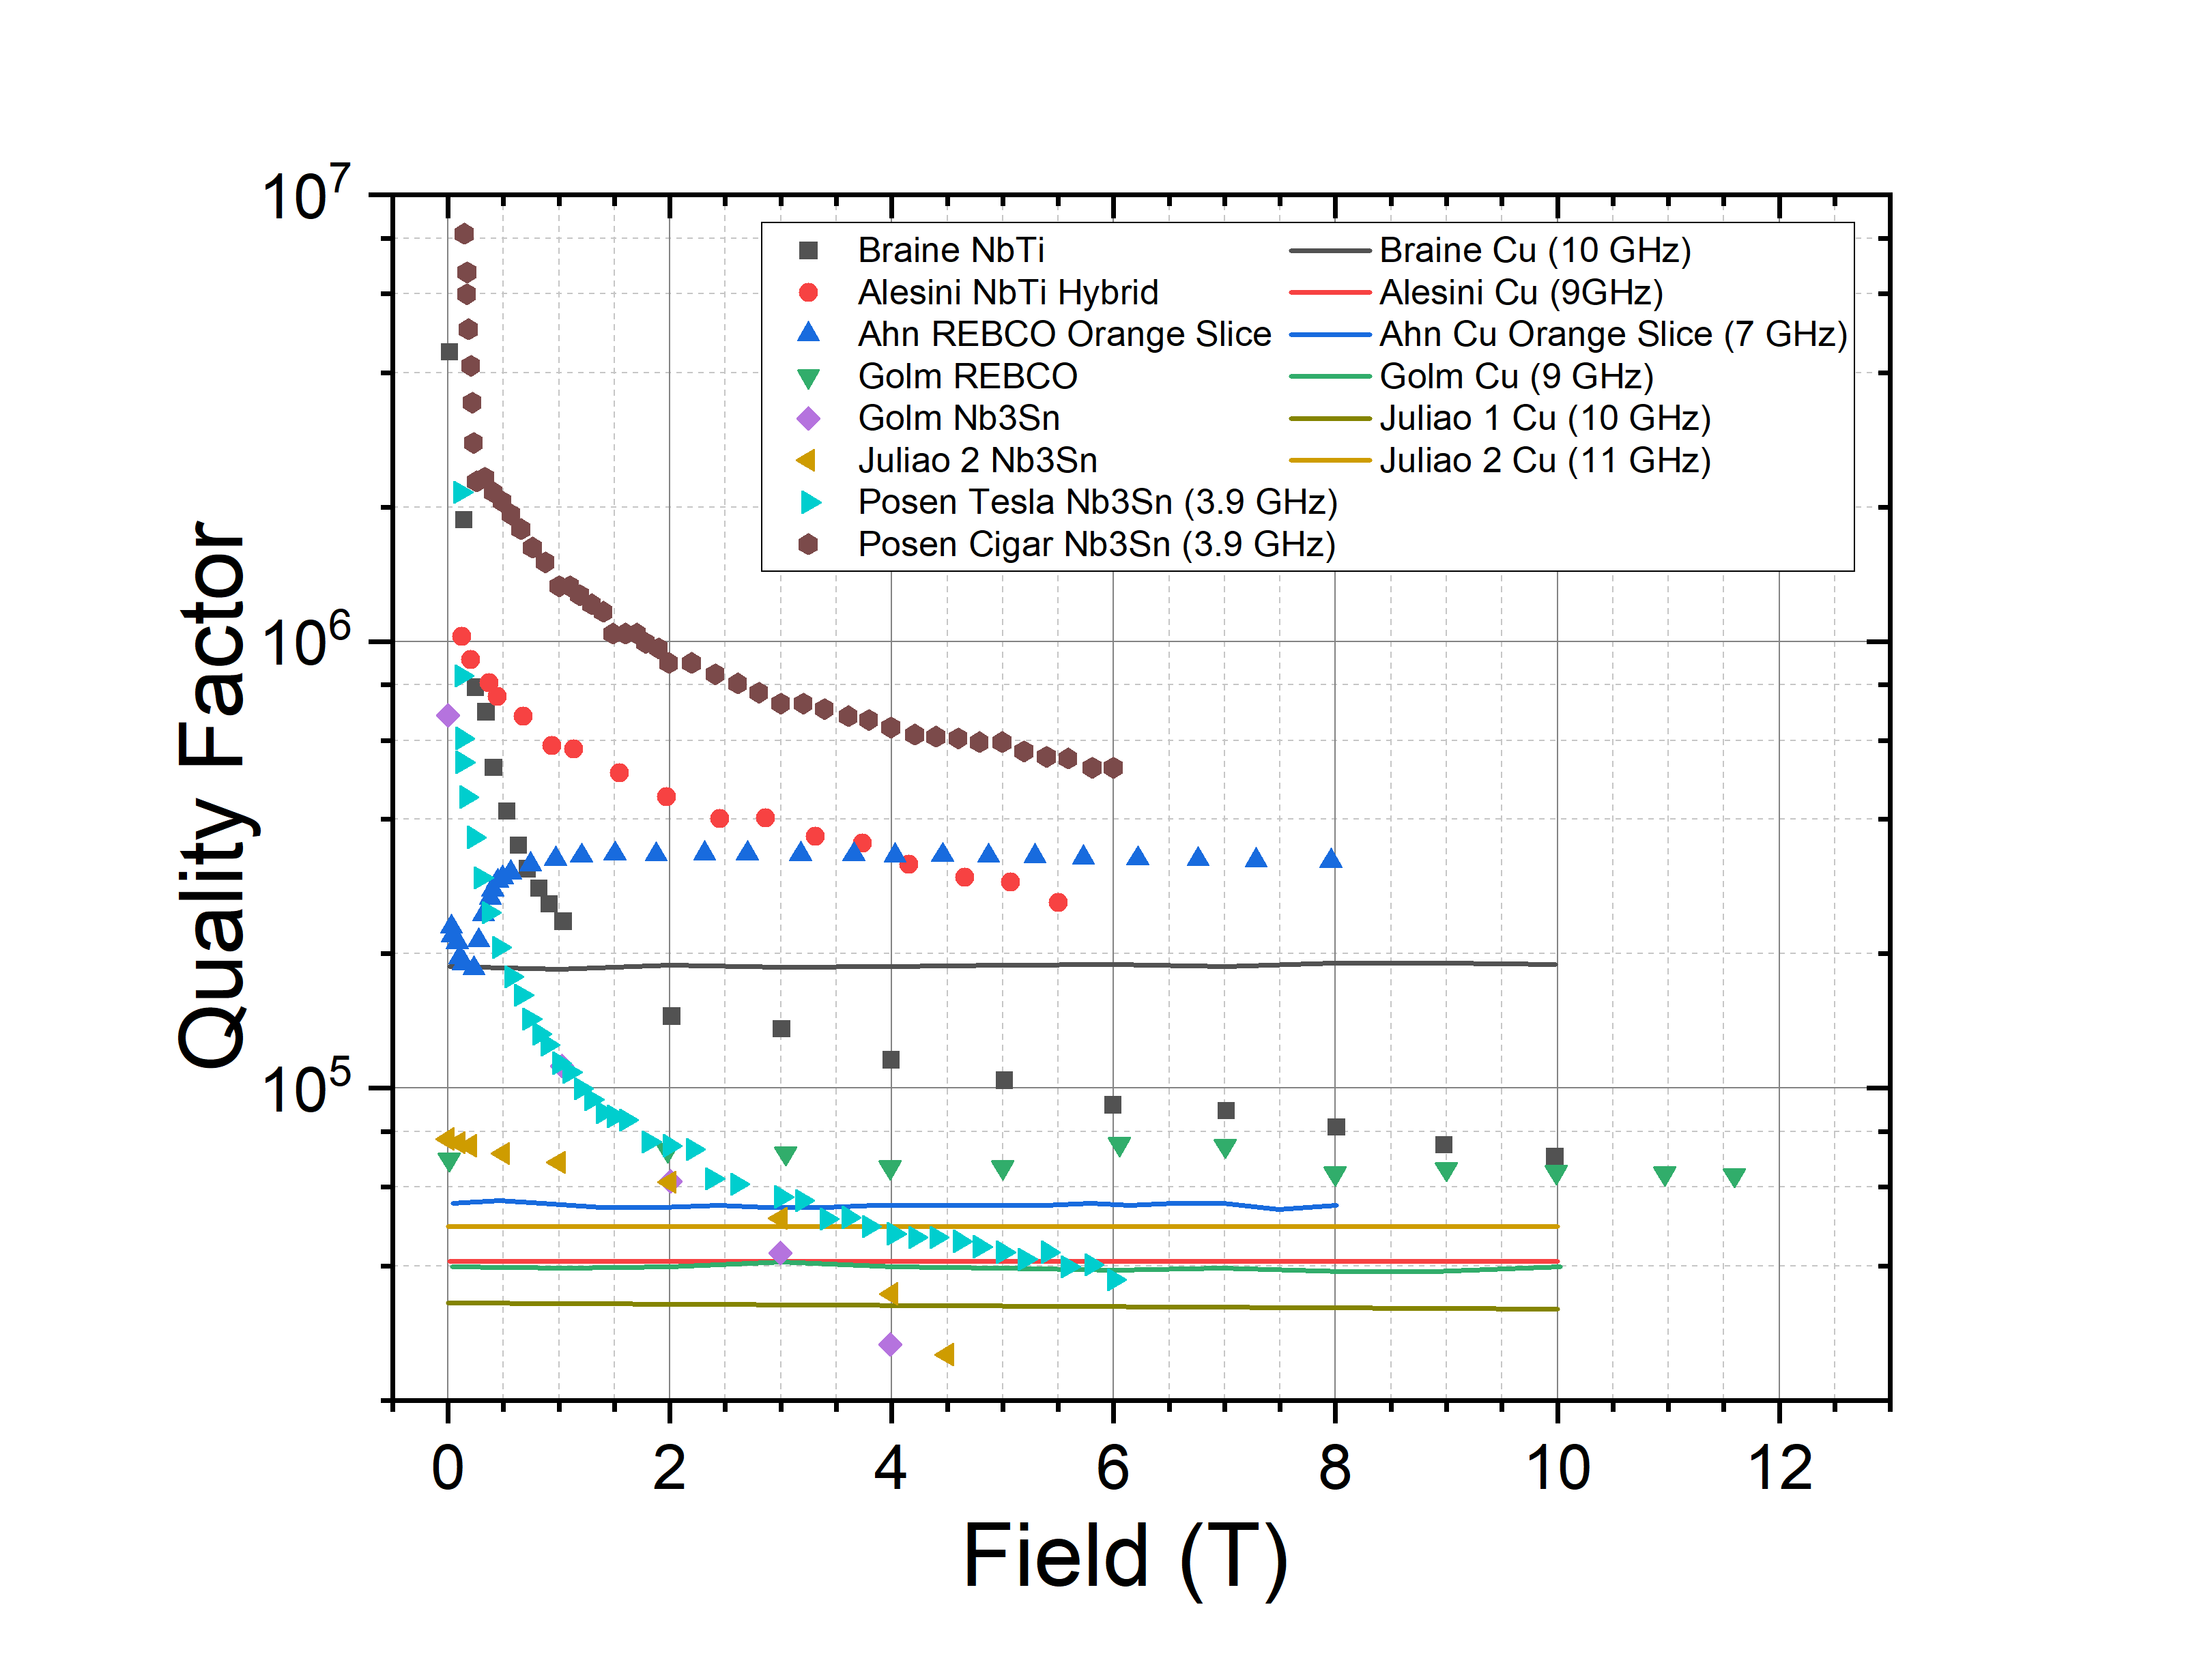
\includegraphics[width=\textwidth]{images/OtherAxionDetector/QvsTAxionPrototypesnew.png}
    \caption[Quality factor vs magnetic field measurements for superconducting axion detector prototypes.]{Quality factor vs magnetic field measurements for superconducting axion detector prototypes. All cavities, except the Posen cavities, had a comparison Cu cavity with the same geometry. The cavities have different frequencies, so data points cannot be compared directly~\cite{ahnSuperconductingCavityHigh2020, Braine:2024nzi, posenNb3SnSuperconductingRadiofrequency2022, Golm:2021ooj, Alesini:2019ajt}.}
    \label{fig:axionprototypes}
\end{figure}

Chapters 1, 2, and 3 explained why an axion haloscope is placed in a large magnetic field. It was also explained why a superconducting cavity (compared to the present copper cavities) increases the scan rate, allowing faster probing across the broad range of possible axion masses. It is argued in Chapter 5 that the available superconducting ductile metal cavities (Bulk Nb) and alloys (NbTi) are not suitable for axion detectors because their maximum upper critical field lies at or below the fields being employed in existing and planned axion searches. This chapter surveys superconductor axion detector prototypes developed for high field and high $Q$, as summarized in the $Q$ vs $B$ plot in Fig.~\ref{fig:axionprototypes}. 

%This chapter also points out the difficulties encountered by many groups in fabricating reproducible cavities meeting the needs of dark matter searches.

%In this chapter, a cavity concept is proposed that implements the material science understanding presented in Chapter 5 and produces a realistic system by which RF properties can be measured in magnetic fields relevant to dark matter searches. Collaborative efforts within the accelerator field are underway to address the specific challenge posed by superconductors in axion-detection applications. 







%To upgrade a resonating cavity from normal conducting to superconducting in a high magnetic field environment, $H_c$ must be kept to a minimum. Dissipative heating can break down superconductivity, leading to decay in the quality factor. The superconducting radio frequency (SRF) accelerator community uses cavities at micro-Tesla magnetic fields while maximizing the RF current. They must keep the surface field below $H_{\text{sh}}$ so the cavity doesn't quench. If a vortex is present in high-RF current cavities (high $E_{\text{acc}}$), the magnetic field lines will experience a large Lorentz force, causing dissipative flux flow and eventually a full thermal breakdown, leading to a quench.

%Resonating cavities for axion detection in high static magnetic fields are in a very different case. The cavity has very low RF power and a strong multi-tesla static magnetic field. This pushes the interest regime above $H_{\text{sh}}$, below $H_{c2}$. The vortices have almost filled the sample at this field, but experience only a small Lorentz force. This small force is ineffective at depinning the vortices, but they will oscillate around their equilibrium position, causing small amounts of dissipation~\cite{campbellResponsePinnedFlux1969}. As the dynamics between pinning and Lorentz forces change, the cavity will experience different loss mechanisms compared to the high-RF accelerating case. Nb-Ti~\cite{leeNiobiumTitaniumSuperconductingWires2001}, Nb$_3$Sn~\cite{sanabriaNewUnderstandingHeat, Tarantini:2021cum}, and REBCO~\cite{paidpilliDevelopmentREBaCuOSuperconductors2022} are materials that have undergone engineering with a high field in mind to increase $H_{c2}$ for magnet design applications~\cite{cooleyChallengesOpportunitiesAssure2022}. Groups have made recent progress using these materials for high-field cavity applications: Nb$_3$Sn\cite{Posen:2022tbs} and REBCO~\cite{ahnSuperconductingCavityHigh2020},\cite{Ahn:2021fgb}, and Nb-Ti~\cite{FirstQUAXGalactic2020}
    
    \section{Nb-Ti Cavities}

    NbTi's upper critical field is too low for this material to be applicable for planned high-field applications. Prior experiments conducted at lower magnetic fields~\cite {ADMX:2023rgo} and development efforts with easy-to-fabricate Nb-Ti help us understand the dependence of $Q$ on the magnetic field for a given superconducting surface orientation with respect to the magnetic field.

    \subsection{ADMX Nb-Ti Cavity}
    
    ADMX currently uses pure copper cavities, but recent work has fabricated a bulk NbTi superconducting cavity, which has been shown to increase sensitivity by $10\times$ compared to Cu at zero field~\cite{Braine:2022qal}. 
    
    \begin{figure}[htb]        
        \centering
        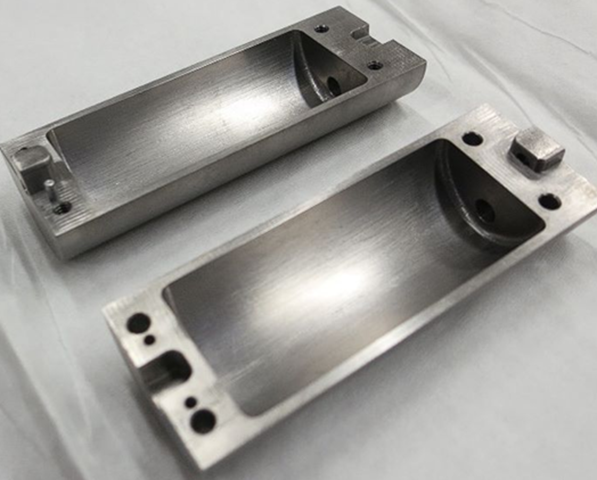
\includegraphics[width=.5\textwidth]{images/OtherAxionDetector/TomNbTi.png}
        \caption{NbTi Bulk Cavity~\cite{Braine:2022qal}.}
        \label{fig:TomNbTi}
    \end{figure}
    
    \citeauthor{Braine:2022qal}~\cite{Braine:2024nzi} modeled and machined a Cu and a bulk NbTi prototype cavity that fits inside a laboratory-size magnet (9~T, 11~GHz, 26~mm diameter). The Cu cavity achieved a quality factor of 180,000 at 2~K, with behavior remaining constant up to 9~T (suggesting that magnetoresistance is not significant). In contrast, the Nb-Ti cavity had a quality factor of 1 million but dropped to 75,000 at 9~T, as seen in~\ref{fig:NbTiQvsT}. A mode decomposition technique introduced by~\cite{Braine:2024nzi}, using different cavity modes and their varying geometric factors, he was able to determine that the NbTi endcaps were more resistive than Cu after just 0.3~T. However, the NbTi wall resistance was at a constant, very low resistance all the way out to 9~T (seen in Fig.~\ref{fig:NbTiendcapsl})~\cite{Braine:2024nzi}. The dependence of surface resistance on magnetic field orientation is explained in Sec.~\ref{sec:campbell}.
    
    \begin{figure}[htb]
        \centering
        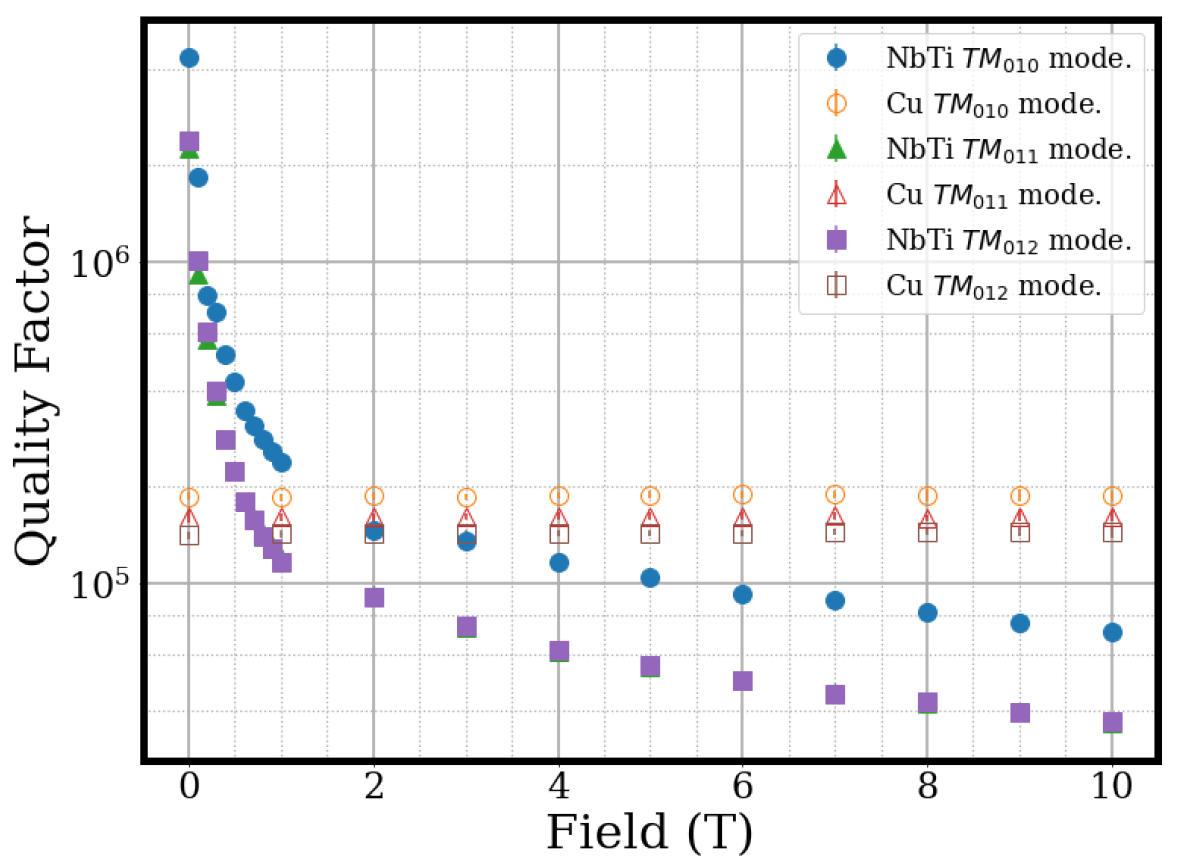
\includegraphics[width=.5\linewidth]{images/OtherAxionDetector/TomQvsFieldCuVSNbTi.png}
        \caption{NbTi versus copper cavity Quality factor vs Magnetic field~\cite{Braine:2022qal}.}
        \label{fig:NbTiQvsT}
    \end{figure}
    
    \begin{figure}[htb]
        \centering
        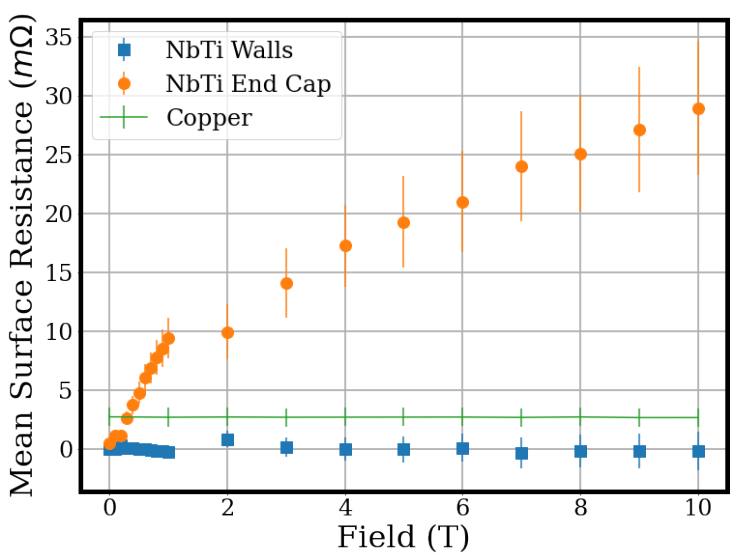
\includegraphics[width=0.5\linewidth]{images/OtherAxionDetector/TomNbTiwallEndcapCu.png}
        \caption{NbTi surface resistance for both the walls and end caps calculated using a mode decomposition technique, compared to the copper cavity resistance~\cite{Braine:2022qal}.}
        \label{fig:NbTiendcapsl}
    \end{figure}
    \FloatBarrier

    \subsection{European Nb-Ti Cavity}
    
    A European group coated a 7 and 9~GHz Cu cavity with a NbTi film~\cite{Alesini:2019ajt, marconatoNbTiThinFilmSRF2024}. The cavity geometry was optimized for minimal magnetic field components perpendicular to the walls, using tapered normal conducting endcaps. This design masked the endcaps during deposition, allowing for a hybrid design with NbTi-coated walls and Cu endcaps. With this optimized design, the quality factor reached $10^6$ at zero field and $10^5$ up to 9~T for the best 7~GHz cavity. 
    
    \begin{figure}[H]        
        \centering
        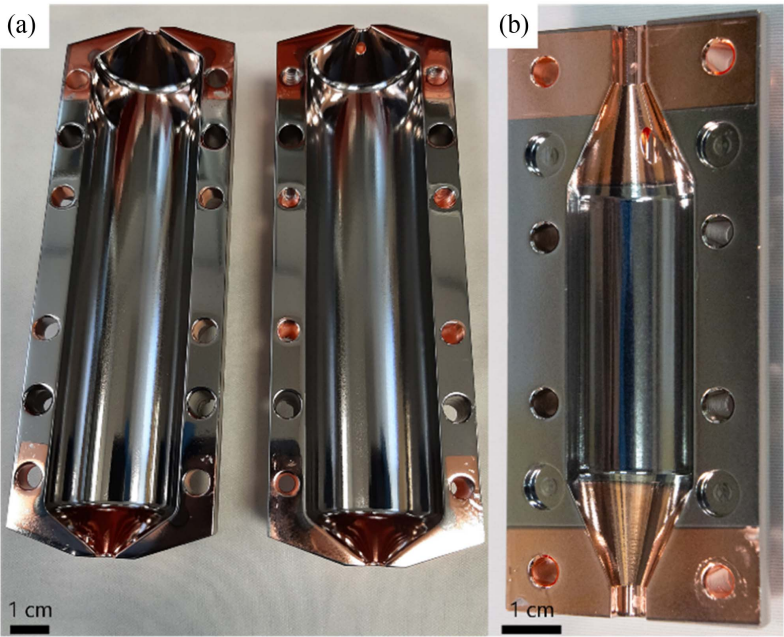
\includegraphics[width=.5\textwidth]{images/OtherAxionDetector/AlesaniNbTi.png}
        \caption{(a) 7-GHz and (b) 9-GHz cavities halves made by the European collaboration~\cite{Alesini:2019ajt, marconatoNbTiThinFilmSRF2024}.}
        \label{fig:AlesaniNbTi}
    \end{figure}
    \FloatBarrier
    
\section{REBCO Cavities}

REBCO cavities are a strong candidate for high-field applications, as they are already optimized in tape form by third-party high-temperature superconductor (HTS) manufacturers. Necessary research related to the fabrication of these REBCO cavities focuses on extracting the REBa$_2$Cu$_3$O$_7$ (RE = rare earth element) superconductor from the materials encapsulating it in the manufactured conductor and soldering the extracted material to the resonating cavity, with the REBCO surface face up. There will be gaps between superconducting tapes, so the REBCO tapes should have the maximum possible width to reduce the number of discontinuities.

\begin{figure}[H]        
    \centering
    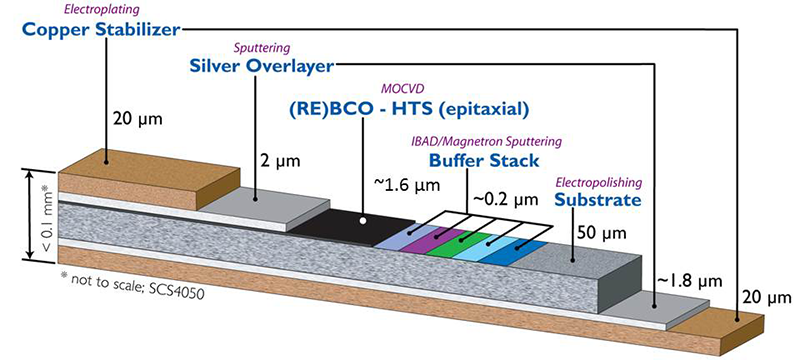
\includegraphics[width=\textwidth]{images/OtherAxionDetector/REBCO.png}
    \caption{A schematic of the REBCO HTS tape’s architecture~\cite{superpowerOurTechnologySuperPower}.}
    \label{fig:REBCO}
\end{figure}


\subsection{South Korean REBCO Cavity}\label{sec:KoreanRebco}


The Institute for Basic Science (IBS) Center for Axion and Precision Physics Research (CAPP) our of Korea, made a REBCO cavity with a stainless steel substrate (Fig.~\ref{fig:AhnREBCO}) for axion detection~\cite{ahnSuperconductingCavityHigh2020}, and achieved the highest quality factor in high magnetic field ($3\times10^5$ at 9~T). They delaminated the REBCO from either the buffer-layer side (between the REBCO superconductor and the Hastelloy tape) or the silver side, and soldered the plated Cu on the outside of the conductor directly to the cavity. REBCO's upper critical field exceeds 100~T at low temperature~\cite{bai40SuperconductingMagnet2020}, which is a possible reason why $Q$ is practically independent of field on the plot in~\ref{fig:axionprototypes}. The REBCO tapes had gaps that aligned with the external magnetic field (solenoid magnet). This led to currents in the TM$_{010}$ mode that do not cross the gaps between tapes.

\begin{figure}[H]        
    \centering
    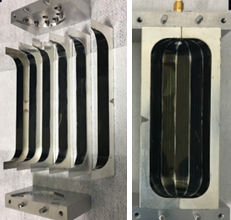
\includegraphics[width=.5\textwidth]{images/OtherAxionDetector/AhnREBCO.png}
    \caption{REBCO orange slice cavity~\cite{ahnSuperconductingCavityHigh2020}.}
    \label{fig:AhnREBCO}
\end{figure}
\FloatBarrier


\subsection{European CERN REBCO Cavity}

\citeauthor{Golm:2021ooj}~\cite{Golm:2021ooj} made a REBCO cavity that showed promising results, with minimal magnetic field degradation out to 9~T (Fig.~\ref{fig:GolmREBCO}). This REBCO cavity has tapes wound circumferentially, perpendicular to the cavity axis. A dipole magnet generated the external magnetic field, so the field remained parallel to the REBCO seams. This prevents the TM$_{010}$ mode currents from crossing the gaps between tapes.

\begin{figure}[H]        
    \centering
    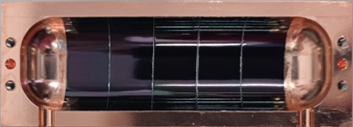
\includegraphics[width=.5\textwidth]{images/OtherAxionDetector/GolmREBCO.png}
    \caption{A REBCO cavity made with the tapes perpendicular to cavity axis~\cite{Golm:2021ooj}.}
    \label{fig:GolmREBCO}
\end{figure}
\FloatBarrier

\section{\texorpdfstring{Nb$_3$Sn}{Nb3Sn} Cavities}

Section~\ref{sec:whynb3sn} explains the rationale for interest in Nb$_3$Sn, which is the material explored in this dissertation.
                        
    \subsection{Sn Vapor \& Optimized Geometry}
    
    \citeauthor{Posen:2022tbs}~\cite{Posen:2022tbs} has taken the Sn vapor method (Sec.~\ref{sec:Snvapordetail}) developed for accelerators and applied it to a specialized cigar-shaped cavity. This shape is designed to reduce magnetic field components perpendicular to the superconducting walls when the external field is aligned with the cavity's long axis. When the DC magnetic field is perpendicular to the superconducting surface, the flux lattice reacts maximally to the Lorentz force from the AC currents, which leads to vortex motion and higher losses (Section~\ref{sec:campbell}). RF testing out to 6~T, comparing the donut-shaped cavity (Fig.~\ref{fig:SamCigarQvsB}) produced by the same process, suggested that the change to a cigar-shaped cavity showed an order-of-magnitude increase in $Q(B)$ (Fig.~\ref{fig:combinedcigartesla}), effective in reducing vortex-induced effects.

    %There was also a tuning rod made for the ADMX collaboration using this Sn vapor method, but it showed poor results and was unable to move when installed in the cavity~\ref{}. 
    
    \begin{figure}[H]         
        \centering
        \begin{subfigure}{0.45\textwidth}
        \centering
        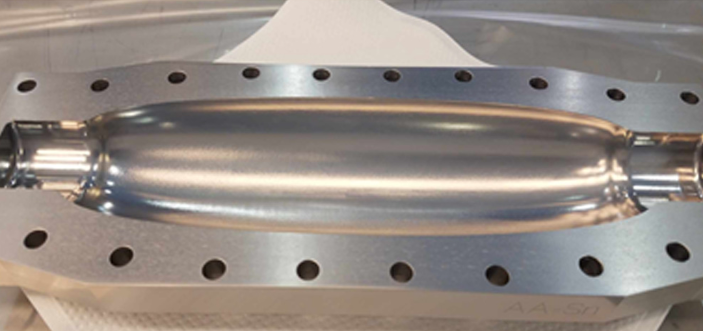
\includegraphics[height = 4cm, angle = 90]{images/OtherAxionDetector/SamCigar.png}
        \caption{}
        \label{fig:Cigar}
        \end{subfigure}
        \begin{subfigure}{0.45\textwidth}
        \centering
        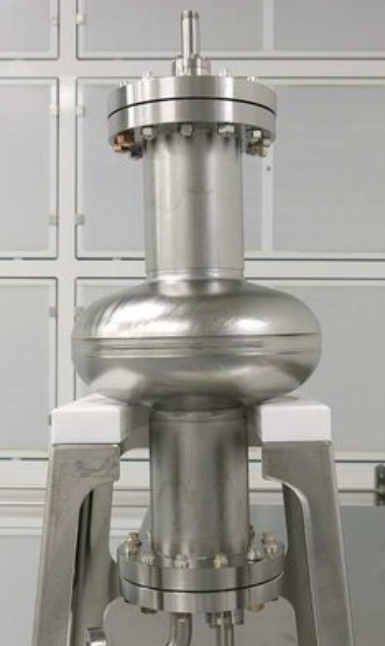
\includegraphics[width = .7\textwidth]{images/intro/Teslacavity.png}
        \caption{}
        \label{fig:Teslacavity}
        \end{subfigure}
        \caption{Two different cavity geometries: a) optimized for high field use called the cigar-shaped cavity at 3.9 GHz~\cite{Posen:2022tbs} and b) a donut-shaped cavity designed for high-velocity particle acceleration at 1.3 GHz~\cite{jiangFeasibilityStudySRF2013}.}
        \label{fig:combinedcigartesla}
    \end{figure}
   
    \begin{figure}[H]        
        \centering
        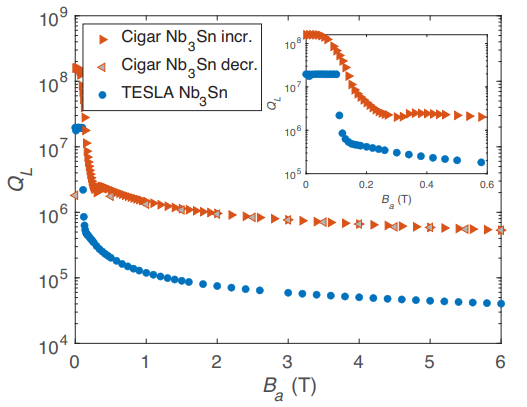
\includegraphics[width=.7\textwidth]{images/OtherAxionDetector/SamCigarQvsB.png}
        \caption[Loaded quality factor versus applied magnetic field for a small 3.9 GHz TESLA cavity shape and the high field designed Cigar cavity.]{Loaded quality factor versus applied magnetic field for a small 3.9 GHz TESLA cavity shape and the high field designed Cigar cavity. Measurements were made in both increasing and decreasing fields for the cigar-shaped cavity~\cite{Posen:2022tbs}.}
        \label{fig:SamCigarQvsB}
    \end{figure}
    \FloatBarrier
        
    \subsection{Stoichiometric \texorpdfstring{Nb$_3$Sn}{Nb3Sn} Target}
        
    Using a similar recipe to the coupon samples from the stoichiometric Nb$_3$Sn target group (discussed in Sec.~\ref{sec:coatings}), \citeauthor{Golm:2021ooj}~\cite{Golm:2021ooj} set out to make a superconducting 9 GHz axion cavity using a Nb$_3$Sn thin film on bulk Cu (Fig.~\ref{fig:GolmNb3sn}) using a similar recipe described in Sec.~\ref{sec:StoichiometricDetail}. Specifically, this experiment used a high-impulse magnetron sputtered (HIPIMS) Ta diffusion barrier (for densification) directly on the Cu substrate, and a stoichiometric Nb$_3$Sn target sputtered at elevated temperature. 
            
    \begin{figure}[H]  
        \centering
        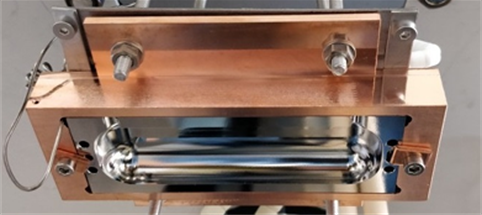
\includegraphics[width=.5\textwidth]{images/OtherAxionDetector/GolmNb3sn.png}
        \caption{The Nb$_3$Sn cavity made by sputtering from a stoichiometric Nb$_3$Sn target~\cite{Golm:2021ooj}.}
        \label{fig:GolmNb3sn}
    \end{figure}
    \FloatBarrier
